\documentclass{article}
% https://github.com/Devinterview-io/docker-interview-questions
% Language setting
% Replace `english' with e.g. `spanish' to change the document language
\usepackage[english]{babel}


% Set page size and margins
% Replace `letterpaper' with `a4paper' for UK/EU standard size
\usepackage[letterpaper,top=2cm,bottom=2cm,left=3cm,right=3cm,marginparwidth=1.75cm]{geometry}

% Useful packages
\usepackage{amsmath}
\usepackage{graphicx}
\usepackage[colorlinks=true, allcolors=blue]{hyperref}
\usepackage{xcolor}
\usepackage[dvipsnames]{xcolor}

\title{GitHub}
\author{SS}

\begin{document}
\maketitle

\begin{abstract}
Your abstract.
\end{abstract}

\section{Introduction}

Just a copy of \href{https://github.com/Devinterview-io/git-interview-questions}{GitQ\&A} \\

\noindent
{\color{red} \rule{\linewidth}{0.5mm}}
\textcolor{red}{1. What is Git and why is it used?} \\
\noindent
{\color{red} \rule{\linewidth}{0.5mm}}


\textcolor{PineGreen}{Docker is a containerization platform that simplifies application deployment by ensuring software and its dependencies run uniformly on any infrastructure, from laptops to server to the clouds.}
\textcolor{PineGreen}{Using Docker allows you to bundle code and dependencies into a container image you can then run on any Docker-compatible environment. This approach is a significant improvement over traditional virtual machines, which are less efficient and come with higher overheads.}\\
\textbf{Key Docker Components:} 
\begin{itemize}
\color{blue}
\item \textbf{Docker Daemon}: A persistent background process that manages and executes containers.
\item \textbf{Docker Engine}: The CLI and API for interacting with the daemon.
\item \textbf{Docker Registry}: A repository for Docker images.
\end{itemize}

\textbf{Core Building Blocks:} 
\begin{itemize}
\color{blue}
\item \textbf{Dockerfile}: A text document containing commands that assemble container image.
\item \textbf{Image}: A standalone, executable package containing everything required to run a piece of software.
\item \textbf{Container}: A runtime instance of an image.
\end{itemize}
\\
\textbf{Virtual Machines vs Docker Containers:} \\
\textbf{Virtual Machines:}
\begin{itemize}
\color{blue}
\item \textbf{Advantages}: 
\begin{itemize}
    \item isolation: VMs run separate OS, providing strict application isolation.
\end{itemize}
\item \textbf{Inefficiencies}: 
\begin{itemize}
    \item Resource Overhead: Each VM requires its OS, consuming RAM, storage and CPU. Running multiple VMs can lead to redundant resource use.
    \item Slow Boot Times: Booting a VM involves starting and entire OS, slowing down deployment.
\end{itemize}
\end{itemize}

\textbf{Containers:}
\begin{itemize}
\color{blue}
\item \textbf{Efficiencies}: 
\begin{itemize}
    \item Resource Optimizations: As containers share the host OS kernel, they are exceptionally lightweight, requiring minimal RAM and storage.
    \item Rapid Deployment: Containers start almost instantaneously, accelerating both development and production.
\end{itemize}
\item \textbf{Isolation Caveats}: 
\begin{itemize}
    \item Application-Level Isolation: While Docker ensures the separation of containers from the host and other containers, it relies on the host OS for underlying resources.
\end{itemize}
\end{itemize}
\\
\textbf{Code Example: Dockerfile} \\
\textcolor{red}{FROM} python:3.8 \\
\textcolor{red}{WORKDIR} /app\\
\textcolor{red}{COPY} requirements.txt requirements.txt\\
\textcolor{red}{RUN} pip install --no-cache-dir -r requirements.txt\\
\textcolor{red}{COPY} . .\\
\textcolor{red}{CMD} ["python", "app.py"] 
\\ 
\textbf{Core Unique Features of Docker:} \\
\begin{itemize}
\color{blue}
\item \textbf{Layered File System}: Docker images are composed of layers, each representing a set of file changes. This structure aids in minimizing image size and optimizing builds.
\item \textbf{Container Orchestration}: Technologies such as Kubernetes and Docker Swarm enable the management of clusters of containers, providing features like load balancing, scaling, and automated rollouts and rollbacks.
\item \textbf{Interoperability}: Docker containers are portable, running consistently across diverse environments. Additionally, Docker complements numerous other tools and platforms, including Jenkins for CI/CD pipelines and AWS for cloud services. 
\end{itemize}
%*********************************************************************
%*********************************************************************
\noindent
{\color{red} \rule{\linewidth}{0.5mm}}
\textcolor{red}{2. How does Git differ from other version control system?} \\
\noindent
{\color{red} \rule{\linewidth}{0.5mm}}
A Docker Image is a lightweight, standalone, and executable software package that includes everything needed to run a piece of software, including the code, a runtime, libraries, environment variables, and configuration files. \\
It provides consistency across environments by ensuring that each instance of an image is identical, a key principle of Docker's build-once-run-anywhere philosophy. \\
\textbf{Image vs. Containers} \\
\begin{itemize}
\color{blue}
\item \textbf{Image}: A static package that encompasses everything the application requires to run.
\item \textbf{Container}: An operating instance of an image, running as a process on the host machine.
\end{itemize}
\textbf{Layered File System} \\
Docker images comprise multiple layers, each representing a distinct file system modification. layers are read-only, and the final container layer is read/write, which allows for efficiency and flexibility. \\   
\textbf{Key Components} \\
\begin{itemize}
\color{blue}
\item \textbf{Operating System}: Traditional images have a full or bespoke OS tailored for the application's needs. Recent developments like "distroless" images, however, focus solely on application dependencies. 
\item \textbf{Application Code}: Your code and files, which are specified during the image build.
\end{itemize}
\textbf{Image Registries} \\
Images are stored in \textbf{Dcoker image registries} like Docker Hub, which provides a central location for image management and sharing. You can download existing images, modify them, and upload modified versions, allowing teams to collaborate efficiently. \\
\textbf{How to build and Image?} \\
\begin{itemize}
\color{blue}
\item \textbf{Dockerfile}: Describes the steps and actions require to set up the image, from selecting the base OS to copying the application code.
\item \textbf{Build Command}: Docker's build command uses the Dockerfile as a blueprint to create the image.
\end{itemize}
\textbf{Advantages of Docker Images} \\
\begin{itemize}
\color{blue}
\item \textbf{Portability}: Docker image ensure consistent behavior across different environments, from development to production.
\item \textbf{Reproducibility}: If you are using the same image, you can expect the same application behaviour.
\item \textbf{Efficiency}: The layered filesystem reduces redundancy and accelerate deployment. 
\item \textbf{Security}: Distinct layers permit granular security control. 
\end{itemize}
\textbf{Code Example: Dockerfile} \\
Here is the Dockerfile: \\


$\#$  Use a base image \\
FROM ubuntu: latest \\

$\#$ Set the working directory \\
WORKDIR /app \\

$\#$ Copy the current directory contents into the container at /app \\
COPY ./app \\

$\#$ Specify the command to run on container start \\
CMD ["/bin/bash"]  \\



\textbf{Best practices for Dockerfiles} \\
\begin{itemize}
\color{blue}
\item Use the official base image if possible.
\item Aim for minimal layers for better efficiency.
\item Regularly update the base image to ensure security and feature updates.
\item Reduce the number of packages installed to minimize security risk.
\end{itemize}

%*********************************************************************
%*********************************************************************
\noindent
{\color{red} \rule{\linewidth}{0.5mm}}
\textcolor{red}{3. What is the difference between Git and GitHub?} \\
\noindent
{\color{red} \rule{\linewidth}{0.5mm}}
Docker images serve as templates for containers, whereas Docker containers are running instances of those images \ref{fig:Docker1}.  \\
\textbf{Key Distinctions}
\begin{itemize}
\color{blue}
\item \textbf{State}: Containers encapsulate both the application code and its runtime environment in a stable and consistent state. In contrast, images are passive and don't change once created.
\item \textbf{Mutable vs Immutable}: Containers like any running process, can modify their state. In contrast, images are immutable and do not change once built.
\item \textbf{Disk Usage}: Containers have both writable layers (such as logs or configuration files) and read-only layers (the image layers), potentially leading to increased disk usage over time. Docker's use of layered storage, however, limits this growth. Images, on the other hand, are solely read-only, meaning each instance based on the same image doesn't consume additional disk space. 
\end{itemize}



\begin{figure}
\centering
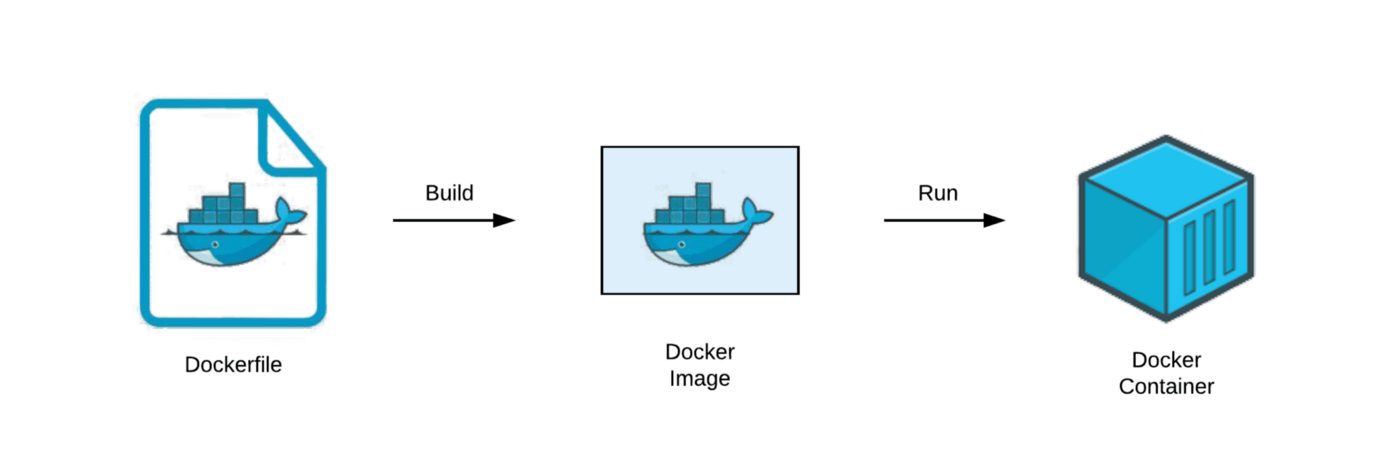
\includegraphics[width=0.95\linewidth]{Docker1.jpg}
\caption{\label{fig:Docker1}TDocker File to Container.}
\end{figure}

\textbf{Practical Demonstration} \\
Here is the code:
\begin{enumerate}
    \item \textbf{Dockerfile} - Define the image:
    \item \textbf{Building an Image} - Use the 'Docker build' command to create the image.
    \item \textbf{Instantiating Containers} - Run the built image with 'docker run' to spawn a container.
    \item \textbf{Viewing Containers} - The 'docker container ls' or 'docker ps' commands display active containers.
    \item \textbf{Modifying Containers} - As an example, you can change the content of a container by entering in via 'docker exec'. \\
    docker exec -it mycontainer /bin/bash
    \item \textbf{Stopping and Removing Containers} - This can be done using the 'docker stop' and 'docker rm' commands otr combined with the '-f' flag. \\
    docker stop mycontainer \\
    docker rm mycontainer 
    \item \textbf{Cleaning up Images} - Remove any unused images to save storage space. \\
    docker image prune -a
\end{enumerate}


%*********************************************************************
%*********************************************************************
\noindent
{\color{red} \rule{\linewidth}{0.5mm}}
\textcolor{red}{4. What is a repository in Git?} \\
\noindent
{\color{red} \rule{\linewidth}{0.5mm}}
A Git repository is a location where all the version-controlled files and their history are stored. It serves as the core component for collaborative and version control windows. \\
\textbf{Key Features:}
\begin{itemize}
    \item \textbf{Distributed }
    \item \textbf{Efficient Storage}
    \item \textbf{Content Integrity}
    \item \textbf{Work Tracking}
\end{itemize}
%*********************************************************************
%*********************************************************************
\noindent
{\color{red} \rule{\linewidth}{0.5mm}}
\textcolor{red}{5. Explain the concept of a \textit{commit} in Git.} \\
\noindent
{\color{red} \rule{\linewidth}{0.5mm}}
One of the defining feature of Docker is its use of Dockerfiles to automate the creation of container images. A Dockerfile is a text document that contains all the commands a user could call on the command line to assemble an image. \\
\textbf{Common Commands}:
\begin{itemize}
    \item \textbf{\textcolor{Red}{FROM}}: \textcolor{PineGreen}{Sets the base image for subsequent build stages}
    \item \textbf{\textcolor{Red}{RUN}}: \textcolor{PineGreen}{Executes commands within the image and then commits the changes}
    \item \textbf{\textcolor{Red}{EXPOSE}}: \textcolor{PineGreen}{Informs Docker that container listens on specific port.}
    \item \textbf{\textcolor{Red}{ENV}}: \textcolor{PineGreen}{Sets environemnt variables.}
    \item \textbf{\textcolor{Red}{ADD/COPY}}: \textcolor{PineGreen}{Adds files from the build context into the image.}
    \item \textbf{\textcolor{Red}{CMD/ENTRYPOINT}}: \textcolor{PineGreen}{Specifies what command to run when the container starts. }
\end{itemize}
%*********************************************************************
%*********************************************************************
\noindent
{\color{red} \rule{\linewidth}{0.5mm}}
\textcolor{red}{6. What is the difference between a \textit{working directory}, \textit{staging area}, and \textit{repository} in \textit{Git}?} \\
\noindent
{\color{red} \rule{\linewidth}{0.5mm}}

%*********************************************************************
%*********************************************************************
\noindent
{\color{red} \rule{\linewidth}{0.5mm}}
\textcolor{red}{7.Define branching in \textit{Git} and its importance?} \\
\noindent
{\color{red} \rule{\linewidth}{0.5mm}}



%*********************************************************************
%*********************************************************************
\noindent
{\color{red} \rule{\linewidth}{0.5mm}}
\textcolor{red}{8. What is a \textbf{HEAD} in \textit{Git}?} \\
\noindent
{\color{red} \rule{\linewidth}{0.5mm}}

%*********************************************************************
%*********************************************************************
\noindent
{\color{red} \rule{\linewidth}{0.5mm}}
\textcolor{red}{9. What does the 'clone' operation in \textit{Git} do?} \\
\noindent
{\color{red} \rule{\linewidth}{0.5mm}}

%*********************************************************************
%*********************************************************************
\noindent
{\color{red} \rule{\linewidth}{0.5mm}}
\textcolor{red}{10. How does \textit{Git} store information?} \\
\noindent
{\color{red} \rule{\linewidth}{0.5mm}}


%*********************************************************************
%*********************************************************************
\noindent
{\color{red} \rule{\linewidth}{0.5mm}}
\textcolor{red}{11. How do you intialize a new Git repository?} \\
\noindent
{\color{red} \rule{\linewidth}{0.5mm}}

%*********************************************************************
%*********************************************************************
\noindent
{\color{red} \rule{\linewidth}{0.5mm}}
\textcolor{red}{12. Explain the purpose of the 'git status' command?} \\
\noindent
{\color{red} \rule{\linewidth}{0.5mm}}


%*********************************************************************
%*********************************************************************
\noindent
{\color{red} \rule{\linewidth}{0.5mm}}
\textcolor{red}{13. What does the 'git add' command do?} \\
\noindent
{\color{red} \rule{\linewidth}{0.5mm}}


%*********************************************************************
%*********************************************************************
\noindent
{\color{red} \rule{\linewidth}{0.5mm}}
\textcolor{red}{14. How do you create a commit in Git?} \\
\noindent
{\color{red} \rule{\linewidth}{0.5mm}}


%*********************************************************************
%*********************************************************************
\noindent
{\color{red} \rule{\linewidth}{0.5mm}}
\textcolor{red}{15. What information is contained in a commit objext in Git?} \\
\noindent
{\color{red} \rule{\linewidth}{0.5mm}}
\end{document}